\usetikzlibrary {automata,positioning}
\scalebox{0.9}{
    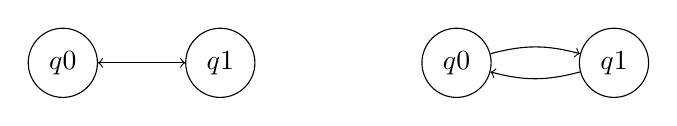
\begin{tikzpicture}[auto]
        \node[state] at (0, 0)(q0){$q0$};
        \node[state] at (2, 0)(q1){$q1$};
        \node[state] at (5, 0)(q2){$q0$};
        \node[state] at (7, 0)(q3){$q1$};

        \path[->]
        (q0)edge (q1)
        (q1)edge (q0)
        (q2)edge [bend left=15] (q3)
        (q3)edge [bend left=15] (q2)
        ;
    \end{tikzpicture}
}

\captionof{figure}{Comparison between implementation(Left) and intended behaviour(Right)}
\label{fig:transitions}